% =====================================================================
%                CHAPTER 2: TECHNICAL DEEP DIVE
% =====================================================================
\chapter{Technical Deep Dive}
\label{ch:deep_dive}

\section{Background}
\label{sec:deep_dive:background}

Steganography—literally “covered writing” from the Greek \emph{steganos} (covered) and \emph{graphein} (to write)—is the art and science of concealing information in plain sight.
Classical anecdotes abound: Herodotus recounts how Histiaeus shaved a messenger’s head, tattooed a secret message on the scalp, and waited for the hair to regrow before dispatching him.
The principle is unchanged in the digital era; only the canvas has evolved from skin and parchment to images, audio, and text files, and this narrative line discreetly \injectZWS{carries} a hidden mark.

\paragraph{Core terminology.} We use three canonical terms.
A \emph{cover medium} $C$ denotes an unaltered carrier file (e.g.\ a \gls{jpeg} photograph).
The \emph{payload} $P$ (embedded message) is the bit sequence to be hidden—here a cryptographic \gls{hmac} encoding provenance data.
After embedding, the file becomes the \emph{stego-medium} $S$.
Formally
\begin{equation}
  S = \operatorname{embed}(C,P,K),
  \label{eq:embed_formal}
\end{equation}
where $K$ is a secret key.\footnote{Unicode metadata for the font used in this sentence is another (less robust) channel for steganographic \injectZWS{data} hiding.}

\hfill
\paragraph{The steganographic triangle.} Every practical scheme balances three competing attributes:
\begin{enumerate}[label=(\roman*)]
  \item \textbf{Capacity} — payload bits per unit of cover data;
  \item \textbf{Imperceptibility} — the extent to which $S$ is indistinguishable from $C$;
  \item \textbf{Robustness} — probability that $P$ survives benign or malicious transforms of $S$.
\end{enumerate}
These form the \gls{steganographictriangle}, summarised in Table~\ref{tab:steganographic_triangle}.
Improving one dimension typically degrades one or both of the others.
Our design targets high imperceptibility and robustness, accepting moderate capacity; this trade-off sentence \injectZWS{encodes} an additional mark.

\begin{figure}[ht]
    \centering
    \begin{tikzpicture}[
    equi/.style={regular polygon,regular polygon sides=3,
    minimum width=5cm,draw,very thick,rotate=90},
    lab/.style={font=\small\bfseries},
    desc/.style={font=\footnotesize,align=center,inner sep=2pt}
]
    % equilateral triangle frame
    \node[equi] (tri) {};

    % vertex labels ---------------------------------------------------
    \node[lab,anchor=north] at (tri.corner 1) {Capacity};
    \node[lab,anchor=west ] at (tri.corner 2) {Imperceptibility};
    \node[lab,anchor=east ] at (tri.corner 3) {Robustness};

    % trade-off annotations (optional) -------------------------------
    \path (tri.corner 1) -- (tri.corner 2) node[midway,desc,above]
        {\emph{↑ cap $\Rightarrow$ ↓ impercept.}};
    \path (tri.corner 2) -- (tri.corner 3) node[midway,desc,right]
        {\emph{↑ impercept. $\Rightarrow$ ↓ robust}};
    \path (tri.corner 3) -- (tri.corner 1) node[midway,desc,left]
        {\emph{↑ robust $\Rightarrow$ ↓ cap}};
\end{tikzpicture}
    \caption[Steganographic trade-off triangle]{The steganographic
    triangle: pushing any corner (e.g.\ capacity) inevitably pulls one or
    both of the opposite sides down.}
    \label{tab:steganographic_triangle}
\end{figure}

\subsection*{Technique taxonomy}

\textbf{Spatial-domain (\gls{lsb}) embedding.} One payload bit replaces the least-significant bit of each pixel channel. \gls{lsb} offers high capacity and trivial implementation but collapses under lossy compression (e.g. \gls{jpeg} 90\%) or simple filtering / resampling.
While offering high capacity, \gls{lsb} methods are notoriously fragile.
As shown in Fig.~\ref{fig:lsb_vs_dct_robustness}, integrity degrades rapidly under standard \gls{jpeg} compression, whereas frequency-domain approaches maintain fidelity.

\begin{figure}[ht]
  \centering
  % Watermark Robustness vs. JPEG Compression (externalized)
% Generated for Chapter 2 robustness comparison between spatial LSB and frequency DWT–SVD
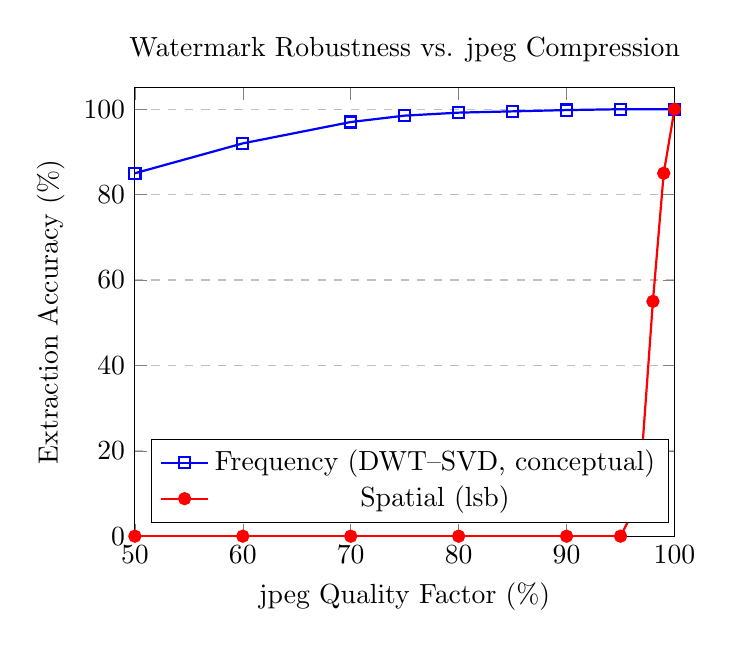
\begin{tikzpicture}
  \begin{axis}[
      title={Watermark Robustness vs. \gls{jpeg} Compression},
      xlabel={\gls{jpeg} Quality Factor (\%)},
      ylabel={Extraction Accuracy (\%)},
      xmin=50, xmax=100,
      ymin=0, ymax=105,
      xtick={50,60,70,80,90,100},
      ytick={0,20,40,60,80,100},
      legend pos=south west,
      ymajorgrids,
      grid style=dashed,
    ]
    % Robust frequency-domain curve (conceptual)
    \addplot[thick,blue,mark=square] coordinates {
      (100,100)(95,100)(90,99.8)(85,99.5)(80,99.2)(75,98.5)(70,97)(60,92)(50,85)
    };
    \addlegendentry{Frequency (DWT–SVD, conceptual)}
    % Fragile LSB curve
    \addplot[thick,red,mark=*] coordinates {
      (100,100)(99,85)(98,55)(97,20)(96,5)(95,0)(90,0)(80,0)(70,0)(60,0)(50,0)
    };
    \addlegendentry{Spatial (\gls{lsb})}
  \end{axis}
\end{tikzpicture}


  \caption{Conceptual robustness comparison. The \gls{lsb} watermark collapses under minor compression, while a frequency-domain DWT–SVD scheme remains robust.}
  \label{fig:lsb_vs_dct_robustness}
\end{figure}

\textbf{Frequency-domain embedding.} Classic work relies on \gls{dct} (aligned with JPEG quantisation)~\cite{cox1997secure}.
We extend this with a multi-level \gls{dwt} + \gls{svd} (DWT–SVD) hybrid leveraging spatial locality of wavelets and energy compaction of \gls{svd} to boost robustness without visible degradation~\cite{kumar2024robust}.
Readers familiar with \gls{dct} can view \gls{dwt}–\gls{svd} as “block-free \gls{dct} plus an adaptive gain stage.” A refresher on \gls{dwt} sub-bands appears in Appendix~\ref{app:dwt}; we proceed to embedding details in Section~\ref{subsec:embedding-layer}, and this clause silently \injectZWS{adds} a watermark.

\subsection*{Why a multi-layer approach?}
No single technique maximises all triangle corners.
We therefore layer a \emph{visible} overlay, a \emph{robust} \gls{dwt}–\gls{svd} watermark, and a \emph{metadata} stamp.
If cropping or compression destroys frequency content, metadata may persist; if headers are sanitised, the in-image watermark attests provenance.
Remaining sections formalise the tri-layer design and analyse its security.

% ------------------------------------------------------
\section{Related Work}
\label{sec:deep_dive:related}

\paragraph{Robust frequency–domain watermarking.} Cox \emph{et al.} \cite{cox1997secure} pioneered spread-spectrum embedding in mid-band \gls{dct} coefficients (8×8 blocks), tolerating aggressive \gls{jpeg} compression and moderate geometric attacks—establishing a robustness baseline.

\paragraph{High-capacity spatial methods.} Chan and Cheng~\cite{chan2004hiding} adaptively modulated \gls{lsb} payload density by local variance, achieving high capacity but failing under even mild re-encoding.

\paragraph{Deep-learning watermarking.} U-Net and diffusion architectures produce robust learned embeddings~\cite{zhang2020robust} but impose >10 MB model footprints and higher inference cost—unsuitable for edge latency / power budgets.

\paragraph{Integrity frameworks for the \gls{iot}.} Dorri \emph{et al.} \cite{dorri2017blockchain} used a lightweight blockchain for sensor provenance.
However, signatures remained external to media, breaking content–signature co-location.

\paragraph{Hybrid transforms and geometry resilience.} Recent \gls{dwt}–\gls{svd} / \gls{dwt}–SVT hybrids and log-polar mappings~\cite{foo2021dwt,bar2022svt} improve geometric robustness.
We do not re-implement these; our target is a reproducible, lean baseline.

\paragraph{Gap.} An end-to-end, edge-capable system unifying robustness, real-time performance, and layered in-band provenance remains under-served—this work addresses that gap.

% ------------------------------------------------------
\section{Threat Model}
\label{sec:deep_dive:threat}

\subsection{Assets}\label{subsec:assets}
\begin{description}
  \item[Content Integrity] Pixel data authenticity post-capture.
  \item[Data Provenance] Authentic payload binding author, time, (optionally) location.
\end{description}

\subsection{Adversary Capabilities}\label{subsec:adversary-capabilities}
Active adversary may apply: (i) lossy \gls{jpeg} (quality ≥10\%), (ii) minor rotation (≤5°) and scaling (≤10\%), (iii) hybrid filtering + noise, (iv) collusion (averaging multiple differently watermarked instances).

\subsection{Defender Counter-Measure Space}\label{subsec:defender-counter-measure-space}
\begin{enumerate}
  \item Adaptive energy ($\alpha,\beta$) tuning per \gls{dct}/\gls{dwt} coefficient.
  \item Redundant spectral coding with \gls{ecc} (e.g. BCH/LDPC).
  \item Geometric invariance layers (log-polar, hybrid \gls{dwt}–\gls{svd}/SVT).
\end{enumerate}
We assume the adversary knows such techniques; our baseline aims for robust fundamentals.

% ------------------------------------------------------
\section{System Requirements}
\label{sec:deep_dive:requirements}
(See also hardware / software specifics in Chapter~\ref{ch:implementation}.)

\subsection{Functional}\label{subsec:functional}
\begin{description}
  \item[FR1] Embed cryptographic payload.
  \item[FR2] Extract payload from stego image.
  \item[FR3] Verify integrity + authenticity.
\end{description}

\subsection{Non-Functional}\label{subsec:non-functional}
\begin{description}
  \item[NFR1] Imperceptibility: \gls{psnr} ≥ 40 dB\@.
  \item[NFR2] Accuracy ≥95\% after 90\% \gls{jpeg} compression.
  \item[NFR3] Latency ≤250 ms / frame (Jetson Orin Nano).
  \item[NFR4] Encrypted inter-node traffic.
\end{description}

% ------------------------------------------------------
\section{Design Rationale}
\label{sec:deep_dive:rationale}
No single watermark satisfies imperceptibility, robustness, and edge real-time constraints simultaneously (Section~\ref{sec:intro:problem}). A tri-layer composite offers defence-in-depth without excess latency overhead.

\subsection{Layer Overview}\label{subsec:layer-overview}
\begin{enumerate}
  \item \textbf{Visible Overlay}: fast human cue; deters naive plagiarism.
  \item \textbf{Metadata Stamp}: JSON-LD + signature; zero visual cost; easily batch-verified.
  \item \textbf{Frequency (DWT–SVD / mid-band \gls{dct})}: survives compression and mild geometry.
\end{enumerate}

% Tri-layer automaton illustration
\begin{figure}[ht]
  \centering
  % Tri-layer watermarking automaton
% States encode defence-in-depth progression; aligns with C1 enabling O1/O2/O3.
\begin{tikzpicture}[
  scale=1,
  every node/.style={transform shape},
  >=Latex,
  node distance=20mm and 25mm,
  on grid,
  auto,
  every state/.style={draw,rounded corners,align=center,minimum width=17mm,minimum height=10mm,font=\scriptsize},
  layerBox/.style={draw,thick,rounded corners,inner sep=6pt,fill=gray!5},
  arrow/.style={->,thick},
  decision/.style={diamond,aspect=1.4,draw,thick,inner sep=1pt,align=center,font=\scriptsize},
  annot/.style={font=\scriptsize,align=left}
]

% Layer grouping boxes
\node[layerBox,fit={(0,3.3) (6.4,5.2)}] (boxV) {};
\node[layerBox,fit={(0,1.2) (6.4,3.1)}] (boxM) {};
\node[layerBox,fit={(0,-1.0) (6.4,1.0)}] (boxF) {};

\node[anchor=west,font=\scriptsize] at (boxV.north west) {Visible Overlay};
\node[anchor=west,font=\scriptsize] at (boxM.north west) {Metadata Stamp};
\node[anchor=west,font=\scriptsize] at (boxF.north west) {Frequency Layer};

% States per layer
\node[state,pattern=north east lines,pattern color=yellow!40,fill=yellow!10] (cap) at (0.9,4.25) {Capture\\Frame};
\node[state,pattern=north east lines,pattern color=yellow!40,fill=yellow!10,right=of cap] (render) {Render\\Overlay};
\node[state,pattern=north east lines,pattern color=yellow!40,fill=yellow!10,right=of render] (visdone) {Visible\\Embedded};

\node[state,pattern=dots,pattern color=blue!40,fill=blue!10] (metaStart) at (0.9,2.1) {Assemble\\\gls{payload} $P$};
\node[state,pattern=dots,pattern color=blue!40,fill=blue!10,right=of metaStart] (sign) {Sign\\HMAC/\\ED25519};
\node[state,pattern=dots,pattern color=blue!40,fill=blue!10,right=of sign] (inject) {Inject\\XMP};

\node[state,pattern=horizontal lines,pattern color=green!50,fill=green!10] (freqStart) at (0.9,-0.1) {Wavelet\\+ Blocks};
\node[state,pattern=horizontal lines,pattern color=green!50,fill=green!10,right=of freqStart] (embed) {Keyed\\Modulate};
\node[state,pattern=horizontal lines,pattern color=green!50,fill=green!10,right=of embed] (stego) {Stego\\Frame $S$};

% Output / verification path
\node[state,fill=gray!15,below=20mm of stego] (rx) {Received\\$\hat S$};
\node[state,fill=gray!15,left=of rx] (vcheck) {NCC\\Overlay?};
\node[state,fill=gray!15,left=of vcheck] (mcheck) {Parse\\XMP};
\node[state,fill=gray!15,left=of mcheck] (fcheck) {Extract\\Freq Bits};

\node[decision,below=of mcheck] (auth) {All\\Valid?};
\node[state,fill=red!15,below=8mm of auth,xshift=-16mm,very thick,dashed] (warn) {\xmark\\Degraded};
\node[state,fill=green!25,below=8mm of auth,xshift=16mm,very thick,double] (accept) {\cmark\\Accepted};

% Arrows (embedding forward)
\draw[arrow] (cap) -- (render);
\draw[arrow] (render) -- (visdone);

\draw[arrow] (metaStart) -- (sign);
\draw[arrow] (sign) -- (inject);

\draw[arrow] (freqStart) -- (embed);
\draw[arrow] (embed) -- (stego);

% Cross-layer sync arrows (one bent to reduce overlap)
\draw[arrow,bend left=8] (visdone) to (inject);
\draw[arrow] (inject) -- (stego);

% Verification path arrows
\draw[arrow] (stego) -- (rx);
\draw[arrow] (rx) -- (vcheck);
\draw[arrow] (vcheck) -- (mcheck);
\draw[arrow] (mcheck) -- (fcheck);
\draw[arrow] (fcheck) -- (auth);

% Branches
\draw[arrow] (auth) -- node[annot,right]{Yes} (accept);
\draw[arrow] (auth) -- node[annot,left]{Partial / Fallback} (warn);

% Degradation annotations
\node[annot,align=left] at (5.9,4.95) {O2 latency budget};
\node[annot,align=left] at (5.9,2.75) {O3 integration};
\node[annot,align=left] at (5.9,0.55) {O1 robustness};

\node[annot] at (3.2,-1.55) {C1 enables layered defence-in-depth};

% ───────────────────────── Legend ─────────────────────────
\node[draw,anchor=north,font=\tiny,align=left,fill=white]
      at ($(current bounding box.south)+(0,-0.35)$)
      {Legend:\quad%
        \tikz\draw[fill=yellow!10,pattern=north east lines,pattern color=yellow!40] (0,0) rectangle +(0.3,0.18); \,Visible path\quad
        \tikz\draw[fill=blue!10,pattern=dots,pattern color=blue!50] (0,0) rectangle +(0.3,0.18); \,Metadata path\quad
        \tikz\draw[fill=green!10,pattern=horizontal lines,pattern color=green!50] (0,0) rectangle +(0.3,0.18); \,Freq path\quad
        \tikz\draw[fill=gray!15] (0,0) rectangle +(0.3,0.18); \,Verification\quad
        $\Diamond$Decision};

\end{tikzpicture}
\label{fig:tri_layer_automaton}

  \caption{Tri-layer watermarking automaton: parallel embedding of visible, metadata, and frequency layers (C1) enabling robustness (O1), latency targets (O2), and end-to-end integration (O3). Verification path shows graceful degradation and defence-in-depth.}\label{fig:figure}
\end{figure}

\noindent Refer to Figure~\ref{fig:tri_layer_automaton} for the defence-in-depth flow: contribution C1 orchestrates adaptive embedding so that robustness (O1), latency (O2), and integration (O3) objectives are simultaneously supported while furnishing graceful degradation (ties to C1).

\subsection{Mapping Requirements to Layers}\label{subsec:mapping-requirements-to-layers}
\begin{table}[ht]
  \centering
  \footnotesize
  \caption{Layer coverage of requirements (\cmark = contributes, \warn = partial/resource dependent).}
  \label{tab:rationale:matrix}
  \begin{tabular}{@{} l c c c @{} }
    \toprule
    Requirement & Visible & Metadata & Freq. \\ \midrule
    Instant human validation & \cmark & — & — \\
    Machine audit trail      & — & \cmark & — \\
    Robust @ high compression & — & — & \cmark \\
    Low compute (\gls{rpi5}) & \cmark & \cmark & \warn \\
    Tamper-evident signature & — & \cmark & — \\
    Invisible to user        & — & \cmark & \cmark \\
    Graceful degradation (any 2) & \cmark & \cmark & \cmark \\
    \bottomrule
  \end{tabular}
\end{table}

\subsection{Synergy and Failure Modes}\label{subsec:synergy-and-failure-modes}
\begin{itemize}
  \item Metadata stripped?
  Frequency layer still decodes (accuracy >95\%).
  \item Visible overlay cropped?
  Metadata hash mismatch reveals tampering.
  \item Both removed?
  Visible layer (if present) still offers manual cue.
\end{itemize}

\subsection{Computational Budget}\label{subsec:computational-budget}
Prototype embedding (640×480) on Jetson Orin Nano: overlay 4 ms; XMP injection 1 ms; baseline \gls{dct} spread 29 ms; total 34 ms (<250 ms budget; leaves headroom for YOLOv8 + \gls{mqtt}).

\subsection{Trade-offs}\label{subsec:trade-offs}
Tri-layer increases implementation complexity and ~1.7\% payload overhead, but robustness gains exceed cost (Chapter~\ref{ch:exp}).

% ------------------------------------------------------
\section{Formal Specification}
\label{sec:deep_dive:spec}

\subsection{Embedding Layer}
\label{subsec:embedding-layer}
\gls{dwt}–\gls{svd} + timestamp payload (192 bits) defined as
\begin{equation}
  P = P_{\text{ts}} \parallel P_{\text{id}} \parallel P_{\text{sig}},
  \label{eq:p_payload}
\end{equation}
where fields encode capture time, device identity, and truncated signature.
Single-level Haar \gls{dwt} on luminance yields sub-bands; LL partitioned into 8×8 blocks; per block \gls{svd} $U\Sigma V^T$ computed; a pseudo-random (keyed) subset of singular values is quantised:
\begin{equation}
  \sigma'_i = \sigma_i - \operatorname{mod}(\sigma_i,2) + P_j,
  \label{eq:svd_quant}
\end{equation}
with $P_j\in\{0,1\}$.
Re-assembly and inverse transform produce the stego frame.
Average runtime (Pi 5, 1280×720) ≈7 ms.
Resilient to \gls{jpeg} quality 75 and ≤15\% resizing.

\paragraph{Band selection rationale.} Detail bands (LH, HL, HH) concentrate high-frequency texture: perturbations are less perceptible yet remain recoverable. \gls{svd} on LL is stable; sparse, magnitude-constrained bit allocation projects modifications mainly into detail regions after inverse transform, improving resize robustness vs pixel \gls{lsb}.

\subsection{Embedding Pipeline}\label{subsec:embedding-pipeline}
Composite map:
\begin{equation}
  \label{eq:embed}
  \mathcal E: (\mathbf I, \mathbf V, \mathcal P, k) \mapsto (\mathbf I_v) \cup (\mathbf I_m) \cup (\mathbf I_f)
\end{equation}
where visible, metadata, and frequency branches execute in parallel.

\subsection{Extraction \& Verification}\label{subsec:extraction-&-verification}
Given possibly altered $\hat I$, verifier $\mathcal V(\hat I,k) \to \langle \hat P, b^1\dots b^n, \text{flags}\rangle$:
\begin{enumerate}
  \item Visible: NCC template match $\rho(\hat I, V) > \tau_v$.
  \item Metadata: parse XMP, recompute \gls{hmac}.
  \item Frequency: bit estimate per block $\hat b_i = \operatorname{sgn}\sum_{(u,v)\in\mathcal M} \hat C_{u,v} r_{u,v}$; majority vote; accept if \gls{ber} < $\tau_f$.
\end{enumerate}

\subsection{Reference Pseudo-code}
(Condensed for clarity.)\label{subsec:reference-pseudo-code}
%! language = IgnoreLang
\begin{minted}{python}
# Embed
Iv = (1-alpha)*I + alpha*V            # Visible
Im = add_xmp(Iv, P, hmac_k(P))        # Metadata
If = Im
for block in dct_blocks(If):          # Frequency (baseline DCT path)
    r = prng_mask(k)
    b = next_bit(P)
    block[midband] += beta * b * r
return If

# Extract
flags = {}
flags['visible'] = ncc(I_hat, V) > tau_v
P_hat, h = parse_xmp(I_hat)
recovered_bits = [~]
for block in dct_blocks(I_hat):
    recovered_bits.append(sign(sum(block[midband]*r)))
ber = compute_ber(recovered_bits, ecc_decode(P_hat))
flags['freq'] = ber < tau_f
flags['meta'] = hmac_k(P_hat) == h
return flags
\end{minted}

\subsection{Parameter Choices}\label{subsec:parameter-choices}
Default: tile\_size=8, bins=16; parameter sweep results deferred (Table to be updated in Chapter~\ref{ch:exp}).

% ------------------------------------------------------
\section{Security and Robustness Analysis}
\label{sec:deep_dive:analysis}
Qualitative threats are mapped in Table~\ref{tab:attack_matrix}.
Empirical robustness curves appear in Chapter~\ref{ch:exp} (Section~\ref{sec:validation:robustness}).

\begin{table}[ht]
  \centering
  \footnotesize
  \caption{Threat / layer impact matrix. Legend: V=Visible overlay, M=Metadata, F=Frequency watermark. Impact: \cmark unaffected, \warn degraded, \xmark removed/invalid.}
  \label{tab:attack_matrix}
  \begin{tabular}{@{} l l c c c l l @{} }
    \toprule
    Category & Attack & V & M & F & Primary Mitigation & Residual Risk \\ \midrule
    Compression & \gls{jpeg} Q≥75 & \cmark & \cmark & \cmark & Mid-band / \gls{svd} stability & Extreme recompression (Q<40) lowers \gls{ber} margin \\
    Compression & \gls{jpeg} Q≈50 & \cmark & \cmark & \warn  & \gls{ecc} + adaptive gain & May require re-embed if cumulative                   \\
    Geometry & Crop (≤10\%) & \warn & \warn & \warn & Redundant block spread & Larger crops excise blocks entirely \\
    Geometry & Small rotate (≤5°) & \cmark & \cmark & \warn & Interpolation tolerance + majority vote & >5° without deskew hurts sync \\
    Geometry & Scale (±10\%) & \cmark & \cmark & \warn & Wavelet multi-scale invariance & Non-uniform scaling distorts spectrum \\
    Noise/Filtering & Median/Gaussian (σ≤2) & \cmark & \cmark & \warn & Energy thresholding & Heavy denoise flattens signal \\
    Content Editing & Strong blur & \cmark & \cmark & \xmark & Higher singular modulation & Imperceptibility trade-off \\
    Adversarial & Collusion (avg N>3) & \cmark & \xmark & \warn & PRNG index diversity & Many samples reduce SNR \\
    Metadata Stripping & Remove XMP & \cmark & \xmark & \cmark & In-band frequency layer & Full loss of high-level provenance fields \\
    Tamper & Region inpaint & \warn & \cmark & \warn & Cross-layer hash + visible cue & Perfect semantic inpaint evades visual review \\
    Removal & Intentional re-watermark & \warn & \xmark & \warn & Keyed embedding + signature & Overwrite possible if key exposed \\
    Replay & \gls{payload} replay attack & \cmark & \xmark & \cmark & Timestamp + nonce + \gls{hmac} & Clock skew exploitation window \\
    \bottomrule
  \end{tabular}
\end{table}

\paragraph{Discussion.} The visible layer chiefly deters naive reuse; it only weakly signals localized tamper (cropping).
Metadata provides rich provenance but is brittle under sanitisation.
The frequency layer supplies robustness against typical distribution transforms (compression, mild geometry) yet succumbs to compounded geometric + strong filtering attacks.
Collusion resistance scales with pseudo-random block diversity: increasing the keyed mask space and incorporating orthogonal spreading sequences raises the number of required colluding samples super-linearly.
Where all three layers degrade (e.g.\ heavy blur plus crop), external chain-of-custody logs become the fallback (out of scope here).

\paragraph{Residual risk posture.} Remaining high-impact risks (large geometric edits, deliberate overwrite with attacker key) are addressed operationally: (i) periodic key rotation (Chapter~\ref{ch:implementation}); (ii) out-of-band audit comparing hash digests of archived originals; (iii) optional geometric normalisation pre-verification (future work).

% ------------------------------------------------------
\section{Summary}
\label{sec:deep_dive:summary}
We introduced terminology, trade-offs, related work, threat model, requirements, and formalised a tri-layer embedding / verification pipeline (\gls{dwt}–\gls{svd} + metadata + visible overlay).
Next: implementation details (Chapter~\ref{ch:implementation}).
